\documentclass{standalone}
\usepackage{tikz}
\usetikzlibrary{patterns, positioning}

\begin{document}
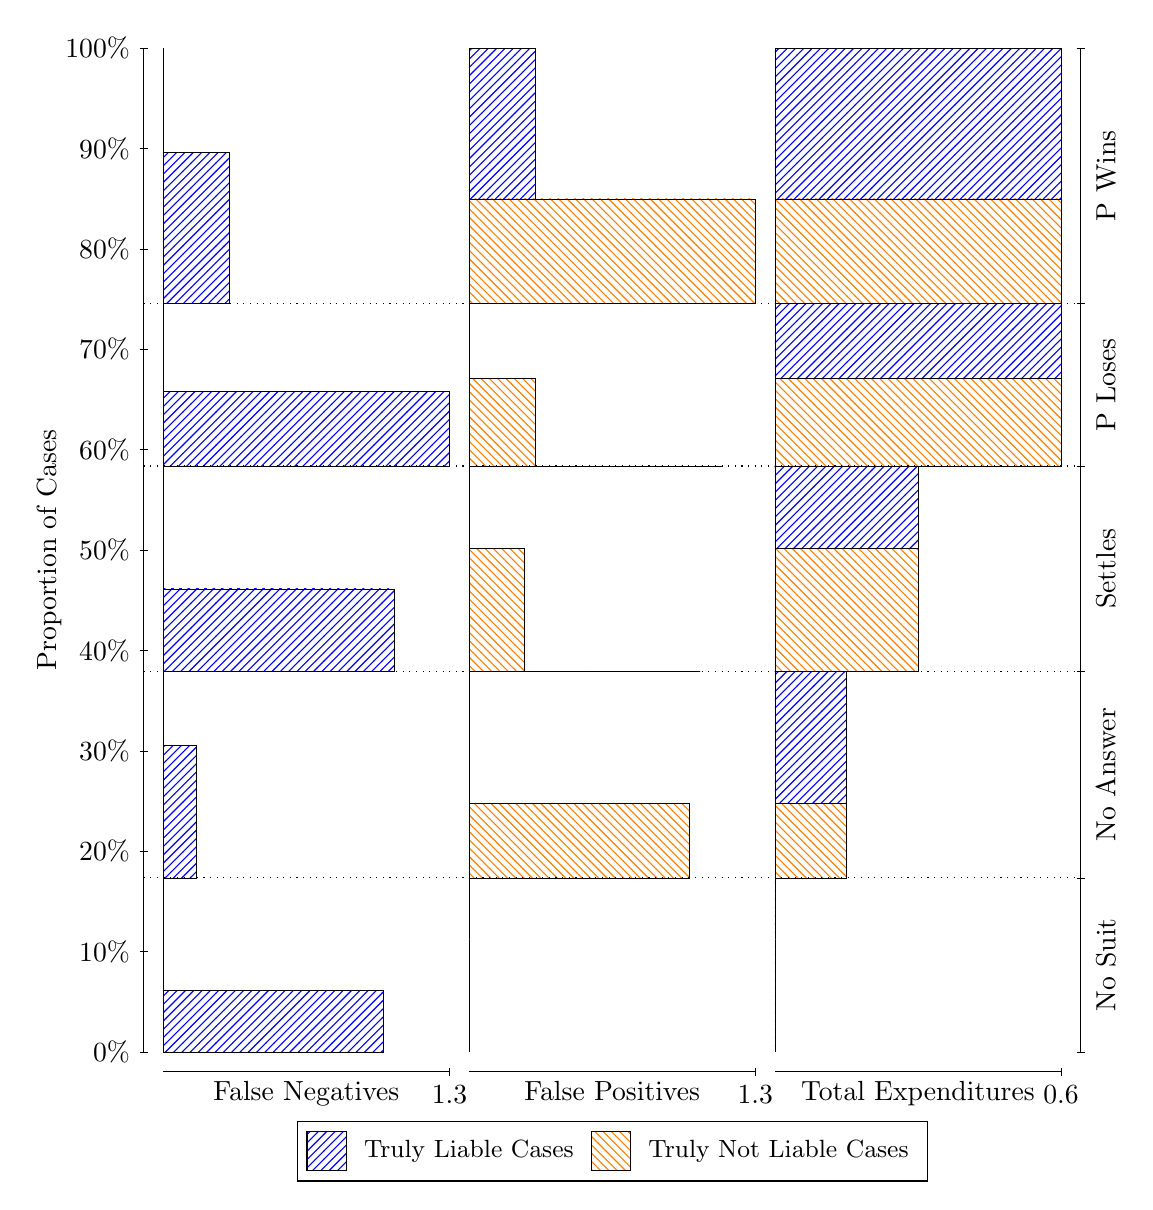
\begin{tikzpicture}
\draw[black, very thin] (1.5,1.75) -- (1.5,14.5);
\node[rotate=90, anchor=center] at (0.3, 8.125) {Proportion of Cases};
\draw[black, very thin] (1.45,1.75) -- (1.55,1.75);
\node[anchor=east] at (1.45, 1.75) {0\%};
\draw[black, very thin] (1.45,3.025) -- (1.55,3.025);
\node[anchor=east] at (1.45, 3.025) {10\%};
\draw[black, very thin] (1.45,4.3) -- (1.55,4.3);
\node[anchor=east] at (1.45, 4.3) {20\%};
\draw[black, very thin] (1.45,5.575) -- (1.55,5.575);
\node[anchor=east] at (1.45, 5.575) {30\%};
\draw[black, very thin] (1.45,6.85) -- (1.55,6.85);
\node[anchor=east] at (1.45, 6.85) {40\%};
\draw[black, very thin] (1.45,8.125) -- (1.55,8.125);
\node[anchor=east] at (1.45, 8.125) {50\%};
\draw[black, very thin] (1.45,9.4) -- (1.55,9.4);
\node[anchor=east] at (1.45, 9.4) {60\%};
\draw[black, very thin] (1.45,10.675) -- (1.55,10.675);
\node[anchor=east] at (1.45, 10.675) {70\%};
\draw[black, very thin] (1.45,11.95) -- (1.55,11.95);
\node[anchor=east] at (1.45, 11.95) {80\%};
\draw[black, very thin] (1.45,13.225) -- (1.55,13.225);
\node[anchor=east] at (1.45, 13.225) {90\%};
\draw[black, very thin] (1.45,14.5) -- (1.55,14.5);
\node[anchor=east] at (1.45, 14.5) {100\%};

\draw[black, very thin] (13.4,1.75) -- (13.4,14.5);
\draw[black, very thin] (13.35,1.75) -- (13.45,1.75);
\node[anchor=west] at (13.35, 1.75) {};
\draw[black, very thin] (13.35,3.9609) -- (13.45,3.9609);
\node[anchor=west] at (13.35, 3.9609) {};
\draw[black, very thin] (13.35,6.5841) -- (13.45,6.5841);
\node[anchor=west] at (13.35, 6.5841) {};
\draw[black, very thin] (13.35,9.1917) -- (13.45,9.1917);
\node[anchor=west] at (13.35, 9.1917) {};
\draw[black, very thin] (13.35,9.1917) -- (13.45,9.1917);
\node[anchor=west] at (13.35, 9.1917) {};
\draw[black, very thin] (13.35,11.257) -- (13.45,11.257);
\node[anchor=west] at (13.35, 11.257) {};
\draw[black, very thin] (13.35,14.5) -- (13.45,14.5);
\node[anchor=west] at (13.35, 14.5) {};

\draw[black, very thin, pattern color=blue, pattern=north east lines] (1.75,1.75) rectangle (4.5449,2.5293);
\draw[black, very thin, pattern color=orange, pattern=north west lines] (1.75,2.5293) rectangle (1.75,3.9609);
\draw[black, very thin, pattern color=blue, pattern=north east lines] (1.75,3.9609) rectangle (2.1692,5.6402);
\draw[black, very thin, pattern color=orange, pattern=north west lines] (1.75,5.6402) rectangle (1.75,6.5841);
\draw[black, very thin, pattern color=blue, pattern=north east lines] (1.75,6.5841) rectangle (4.6846,7.6319);
\draw[black, very thin, pattern color=blue, pattern=north east lines] (1.75,7.6319) rectangle (4.4051,7.6319);
\draw[black, very thin, pattern color=blue, pattern=north east lines] (1.75,7.6319) rectangle (4.1256,7.6319);
\draw[black, very thin, pattern color=blue, pattern=north east lines] (1.75,7.6319) rectangle (3.8462,7.6319);
\draw[black, very thin, pattern color=blue, pattern=north east lines] (1.75,7.6319) rectangle (3.5667,7.6319);
\draw[black, very thin, pattern color=blue, pattern=north east lines] (1.75,7.6319) rectangle (3.2872,7.6319);
\draw[black, very thin, pattern color=blue, pattern=north east lines] (1.75,7.6319) rectangle (3.0077,7.6319);
\draw[black, very thin, pattern color=blue, pattern=north east lines] (1.75,7.6319) rectangle (2.7282,7.6319);
\draw[black, very thin, pattern color=blue, pattern=north east lines] (1.75,7.6319) rectangle (2.4487,7.6319);
\draw[black, very thin, pattern color=orange, pattern=north west lines] (1.75,7.6319) rectangle (1.75,9.1917);
\draw[black, very thin, pattern color=blue, pattern=north east lines] (1.75,9.1917) rectangle (2.1692,9.1917);
\draw[black, very thin, pattern color=orange, pattern=north west lines] (1.75,9.1917) rectangle (1.75,9.1917);
\draw[black, very thin, pattern color=blue, pattern=north east lines] (1.75,9.1917) rectangle (5.3833,10.144);
\draw[black, very thin, pattern color=orange, pattern=north west lines] (1.75,10.144) rectangle (1.75,11.257);
\draw[black, very thin, pattern color=blue, pattern=north east lines] (1.75,11.257) rectangle (2.5885,13.173);
\draw[black, very thin, pattern color=orange, pattern=north west lines] (1.75,13.173) rectangle (1.75,14.5);
\draw[black, very thin, pattern color=orange, pattern=north west lines] (5.6333,1.75) rectangle (5.6333,3.1816);
\draw[black, very thin, pattern color=blue, pattern=north east lines] (5.6333,3.1816) rectangle (5.6333,3.9609);
\draw[black, very thin, pattern color=orange, pattern=north west lines] (5.6333,3.9609) rectangle (8.4282,4.9047);
\draw[black, very thin, pattern color=blue, pattern=north east lines] (5.6333,4.9047) rectangle (5.6333,6.5841);
\draw[black, very thin, pattern color=orange, pattern=north west lines] (5.6333,6.5841) rectangle (8.5679,6.5841);
\draw[black, very thin, pattern color=orange, pattern=north west lines] (5.6333,6.5841) rectangle (8.2885,6.5841);
\draw[black, very thin, pattern color=orange, pattern=north west lines] (5.6333,6.5841) rectangle (8.009,6.5841);
\draw[black, very thin, pattern color=orange, pattern=north west lines] (5.6333,6.5841) rectangle (7.7295,6.5841);
\draw[black, very thin, pattern color=orange, pattern=north west lines] (5.6333,6.5841) rectangle (7.45,6.5841);
\draw[black, very thin, pattern color=orange, pattern=north west lines] (5.6333,6.5841) rectangle (7.1705,6.5841);
\draw[black, very thin, pattern color=orange, pattern=north west lines] (5.6333,6.5841) rectangle (7.1705,6.5841);
\draw[black, very thin, pattern color=orange, pattern=north west lines] (5.6333,6.5841) rectangle (6.891,6.5841);
\draw[black, very thin, pattern color=orange, pattern=north west lines] (5.6333,6.5841) rectangle (6.6115,6.5841);
\draw[black, very thin, pattern color=orange, pattern=north west lines] (5.6333,6.5841) rectangle (6.3321,8.1438);
\draw[black, very thin, pattern color=blue, pattern=north east lines] (5.6333,8.1438) rectangle (5.7731,8.1438);
\draw[black, very thin, pattern color=blue, pattern=north east lines] (5.6333,8.1438) rectangle (5.6333,9.1917);
\draw[black, very thin, pattern color=orange, pattern=north west lines] (5.6333,9.1917) rectangle (8.8474,9.1917);
\draw[black, very thin, pattern color=blue, pattern=north east lines] (5.6333,9.1917) rectangle (6.0526,9.1917);
\draw[black, very thin, pattern color=orange, pattern=north west lines] (5.6333,9.1917) rectangle (6.4718,10.305);
\draw[black, very thin, pattern color=blue, pattern=north east lines] (5.6333,10.305) rectangle (5.6333,11.257);
\draw[black, very thin, pattern color=orange, pattern=north west lines] (5.6333,11.257) rectangle (9.2667,12.584);
\draw[black, very thin, pattern color=blue, pattern=north east lines] (5.6333,12.584) rectangle (6.4718,14.5);
\draw[black, very thin, pattern color=orange, pattern=north west lines] (9.5167,1.75) rectangle (9.5167,3.1816);
\draw[black, very thin, pattern color=blue, pattern=north east lines] (9.5167,3.1816) rectangle (9.5167,3.9609);
\draw[black, very thin, pattern color=orange, pattern=north west lines] (9.5167,3.9609) rectangle (10.425,4.9047);
\draw[black, very thin, pattern color=blue, pattern=north east lines] (9.5167,4.9047) rectangle (10.425,6.5841);
\draw[black, very thin, pattern color=orange, pattern=north west lines] (9.5167,6.5841) rectangle (11.333,6.5841);
\draw[black, very thin, pattern color=blue, pattern=north east lines] (9.5167,6.5841) rectangle (11.333,6.5841);
\draw[black, very thin, pattern color=orange, pattern=north west lines] (9.5167,6.5841) rectangle (11.333,8.1438);
\draw[black, very thin, pattern color=blue, pattern=north east lines] (9.5167,8.1438) rectangle (11.333,9.1917);
\draw[black, very thin, pattern color=orange, pattern=north west lines] (9.5167,9.1917) rectangle (11.333,9.1917);
\draw[black, very thin, pattern color=blue, pattern=north east lines] (9.5167,9.1917) rectangle (11.333,9.1917);
\draw[black, very thin, pattern color=orange, pattern=north west lines] (9.5167,9.1917) rectangle (11.333,9.1917);
\draw[black, very thin, pattern color=blue, pattern=north east lines] (9.5167,9.1917) rectangle (11.333,9.1917);
\draw[black, very thin, pattern color=orange, pattern=north west lines] (9.5167,9.1917) rectangle (13.15,10.305);
\draw[black, very thin, pattern color=blue, pattern=north east lines] (9.5167,10.305) rectangle (13.15,11.257);
\draw[black, very thin, pattern color=orange, pattern=north west lines] (9.5167,11.257) rectangle (13.15,12.584);
\draw[black, very thin, pattern color=blue, pattern=north east lines] (9.5167,12.584) rectangle (13.15,14.5);
\draw[black, dotted] (1.5,3.9609) -- (13.4,3.9609);
\draw[black, dotted] (1.5,6.5841) -- (13.4,6.5841);
\draw[black, dotted] (1.5,9.1917) -- (13.4,9.1917);
\draw[black, dotted] (1.5,9.1917) -- (13.4,9.1917);
\draw[black, dotted] (1.5,11.257) -- (13.4,11.257);
\draw[black, very thin] (1.75,1.5) -- (5.3833,1.5);
\node[anchor=north] at (3.5667, 1.5) {False Negatives};
\draw[black, very thin] (5.3833,1.45) -- (5.3833,1.55);
\node[anchor=north] at (5.3833, 1.45) {1.3};

\draw[black, very thin] (5.6333,1.5) -- (9.2667,1.5);
\node[anchor=north] at (7.45, 1.5) {False Positives};
\draw[black, very thin] (9.2667,1.45) -- (9.2667,1.55);
\node[anchor=north] at (9.2667, 1.45) {1.3};

\draw[black, very thin] (9.5167,1.5) -- (13.15,1.5);
\node[anchor=north] at (11.333, 1.5) {Total Expenditures};
\draw[black, very thin] (13.15,1.45) -- (13.15,1.55);
\node[anchor=north] at (13.15, 1.45) {0.6};

\node[black, centered, rotate=90] at (13.72, 2.8554) {No Suit};
\node[black, centered, rotate=90] at (13.72, 5.2725) {No Answer};
\node[black, centered, rotate=90] at (13.72, 7.8879) {Settles};

\node[black, centered, rotate=90] at (13.72, 10.224) {P Loses};
\node[black, centered, rotate=90] at (13.72, 12.878) {P Wins};

\draw (7.449999999999999,1.5) node[draw=none] (baseCoordinate) {};
\begin{scope}[align=center]
        \matrix[scale=0.5, draw=black, below=0.5cm of baseCoordinate, nodes={draw}, column sep=0.1cm]{
            \node[rectangle, draw, minimum width=0.5cm, minimum height=0.5cm, pattern=north east lines, pattern color=blue] {}; &
            \node[draw=none, font=\small] (B) {Truly Liable Cases}; &
            \node[rectangle, draw, minimum width=0.5cm, minimum height=0.5cm, pattern=north west lines, pattern color=orange] {}; &
            \node[draw=none, font=\small] (B) {Truly Not Liable Cases}; \\
            };
\end{scope}

\end{tikzpicture}
\end{document}